% Use style package recommended by conference.
\documentclass[letterpaper,single,9pt]{article}

\usepackage[all=normal, paragraphs, indent, lists, floats, sections, title]{savetrees}

\usepackage{epsfig}
\usepackage{graphicx}
\usepackage{subfigure}
\usepackage{amsmath,amssymb}
\usepackage{color}
\usepackage[hyphens]{url}
\usepackage{listings}
\usepackage[normalem]{ulem}
\usepackage{floatrow}
\usepackage{xspace}
\usepackage{amsmath}
\usepackage{enumitem}
\usepackage{booktabs}
\usepackage[utf8]{inputenc}
\usepackage{authblk}
\usepackage{hyperref}
\usepackage{algorithm, algpseudocode}
\usepackage{fancyvrb}
\usepackage{cprotect}
\usepackage{mdframed}
\usepackage{array}
\usepackage{cite}
\usepackage{multirow}
\usepackage{caption}
\usepackage[usenames,dvipsnames]{xcolor}
\begin{document}
\title{COMS W4771 - Machine Learning 1st Exersice}

  \author{ {\rm Georgios Koloventzos - gk2409} \\ }

\maketitle

\section{Problem 1}

The exercise at the beginning asks for the best degree using some empirical risk.
Function polyreg does exactly this when 3 arguments are given.
So for having some empirical results we will run the polyreg function
in a variety of degrees. In general we use the degrees from 1 to 50.
We choose this as the final plot it resembles the one in the example.

So using Matlab code we do
\begin{verbatim}
emp_err=zeros(D,1);
for i=1:50
   [emp_err(i),emp_mod] = polyreg(x,y,i);
end
best-emp-d=find(emp_err==min(emp_err))
\end{verbatim}

This snipset of code will give us in the best-emp-d variable the 
index of the lowest error which is the degree of the polynomial.
The result for the empirical is that the lowest error comes with
a 11th degree polynomial.

\begin{figure}[!h]
{
    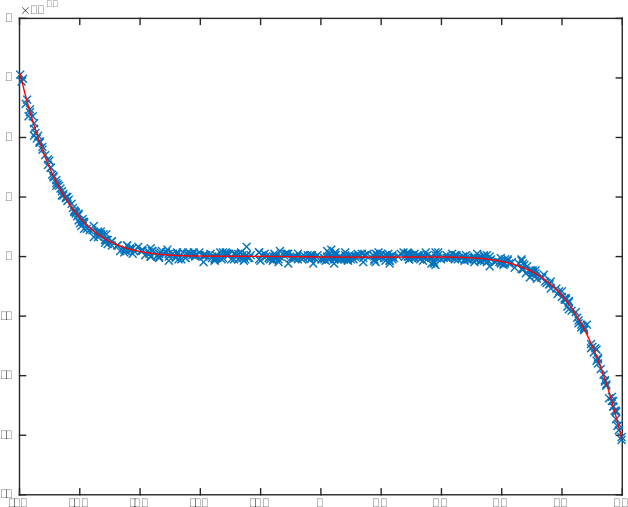
\includegraphics[width=\columnwidth]
    {figures/bestpolu}
    \caption{\footnotesize{\bf} Data with the best polynomial.}
    \label{fig:f}
}
\end{figure}

If we print all the empirical risks that we found we will see
that the lowest error is with the polynomial degree 8,9,10,11
and the ones with degrees 12,13,14,15,16 are really close.
The errors are 0.0113 and 0.0114 respectively.

So that degrees are somehow reasonable.

In order to do 2-fold cross validation we split our data into 2 sets.
I use the randperm function to create an array with the numbers from
1 to 500. This will split the data in 2 random sets. Then we will 
run the polyreg function 2 times one with the 1st set as training and
the 2nd as testing and vice versa. Then we will average the 2 errors
between these 2 runs to give us the best degree of polynomial. From
our empirical measurement I believe that it should be between 8th and
15th degree.

\begin{verbatim}
indx = randperm(length(x));
xTr=zeros(length(x)/2,1);
yTr=zeros(length(x)/2,1);
xTe=zeros(length(x)/2,1);
yTe=zeros(length(x)/2,1);
cross_err_1=zeros(D,1);
cross_err_2=zeros(D,1);
cross_errT_1=zeros(D,1);
cross_errT_2=zeros(D,1);

for i=1:length(x)/2
    xTr(i)=x(indx(i));
    yTr(i)=y(indx(i));
end

for i=length(x)/2+1:length(x)
    xTe(i)=x(indx(i));
    yTe(i)=y(indx(i));
end

for i=1:D
    [cross_err_1(i),cross_mod_1,cross_errT_1(i)] = polyreg(xTr,yTr,i,xTe,yTe);
    [cross_err_2(i),cross_mod_2,cross_errT_2(i)] = polyreg(xTe,yTe,i,xTr,yTr);
end

average_errT=zeros(D,1);
average_err=zeros(D,1);

for i=1:D
    average_err(i)=(cross_err_1(i)+cross_err_2(i))/2;
    average_errT(i)=(cross_errT_1(i)+cross_errT_2(i))/2;
end

best_d=find(average_err==min(average_err))
polyreg(x,y,best_d)

figure(7)
plot((1:50),average_err,(1:50),average_errT)
title('Training and Data error')
xlabel('Degree of Polymomial')
ylabel('Error')
legend('Train Data', 'Test Data')
\end{verbatim}

The result of this procedure varies. This is because the training and
testing data differ in each run. But still at my runs, it is never lower
than 8 or more than 15. This coincides with the empirical risk
we already found.


\section{Problem 2}

The Matlab files for this exercise are \texttt{multireg.m} and \texttt{hm1\_2.m}

I use the least square loss function to penalize in order to use the gradient function that we have from the slides(slide 9, class3x.pdf).

For the 2-fold cross validation I use the same techinque as the Problem 1, dividing the dataset into 2 sets. I use one set as training and the other as test and vice versa. The plot that is created is far from what we have seen in class. In this exercise I split the dataset in half and not in random. The $\lambda$ that minimizes the testing error is 950 (figure \ref{fig:ex2}).
From the plot we can conclude that the our function that does the penalize does not have underfitting (it is too small).

\begin{figure}[!h]
{
    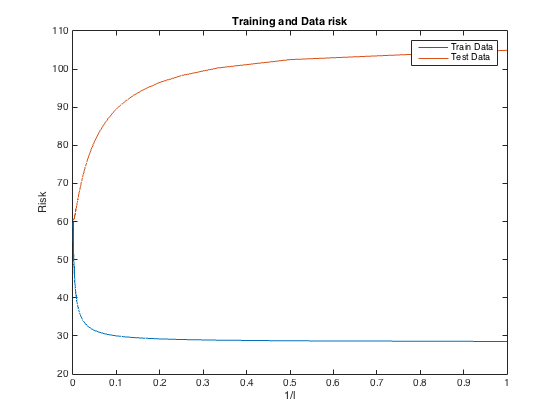
\includegraphics[width=\columnwidth]
    {figures/hm1_2.png}
    \caption{\footnotesize{\bf}Training and Testing Risk}
    \label{fig:ex2}
}
\end{figure} 

\section{Problem 3}
\subsection{1}
\begin{align*}
1-g(x) = 1 - \cfrac{1}{1+\cfrac{1}{{e^x}}} \Leftrightarrow \\
1-g(x) = 1 - \cfrac{1}{\cfrac{e^x + 1}{e^x}} \Leftrightarrow \\
1-g(x) = 1 - \cfrac{e^x}{e^x + 1} \Leftrightarrow \\
1-g(x) = \cfrac{e^x+1-e^x}{e^x+1} \Leftrightarrow \\
1-g(x) = \cfrac{1}{e^x+1} \Leftrightarrow \\
1-g(x) = g(-x)
\end{align*}
\subsection{2}
\begin{align*}
g(x) = \frac{1}{1+e^{-x}} = y \\
y+y*e^{-x} = 1 \Rightarrow \\
e^{-x} = \frac{1-y}{y} \Rightarrow \\
e^x = \frac{y}{1-y} \Rightarrow \\
\ln(e^x) = \ln(\frac{y}{1-y}) \Rightarrow \\
x = \ln(\frac{y}{1-y}) \Rightarrow \\
g^{-1}(x) = \ln(\frac{y}{1-y})
\end{align*}

\section{Problem 4}
Here is the derivations I did in order to an easier function inside
the gradient:

\begin{eqnarray*}
\sum_{i=1}^n \Bigl( \frac{1-y_i}{1-f(x_i;\theta)} - 
\frac{y_i}{f(x_i;\theta)}\Bigr)f'(x_i;\theta) \Leftrightarrow
\sum_{i=1}^n \Bigl( \frac{1-y_i}{1-g(\theta^Tx)} -
\frac{y_i}{g(\theta^Tx)}\Bigr)g'(\theta^Tx) \Leftrightarrow \\
\sum_{i=1}^n \Bigl( \frac{1-y_i}{1-g(\theta^Tx)} -
\frac{y_i}{g(\theta^Tx)}\Bigr)(\theta^Tx)'(g'(\theta^Tx)) \Leftrightarrow
\sum_{i=1}^n \Bigl( \frac{1-y_i}{1-g(\theta^Tx)} -
\frac{y_i}{g(\theta^Tx)}\Bigr)*x*g(\theta^Tx)(1-g(\theta^Tx)) \Leftrightarrow \\
\sum_{i=1}^n \Bigl( (1-y_i)*g(\theta^Tx) - (y_i*(1-g(\theta^Tx))*x\Bigr) \Leftrightarrow
\sum_{i=1}^n \Bigl( (g(\theta^Tx) - y_i)x \Bigr)
\end{eqnarray*}

The Matlab files for this exercise are \texttt{logreg.m} and \texttt{hm1\_4.m}
You can find the Desicion boundary figure \ref{fig:db}. The binary classification error \ref{fig:bce}. The empirical risk figure \ref{ref:er}.
\begin{figure}[!h]
{
    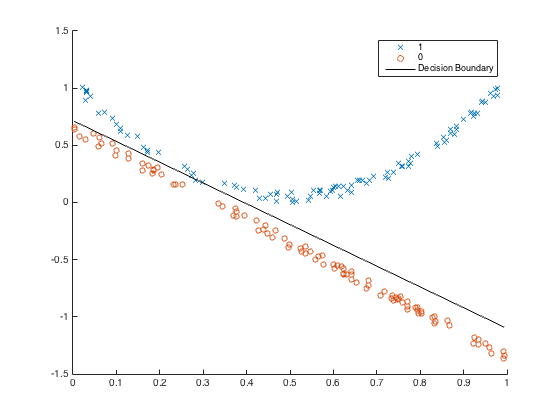
\includegraphics[width=\columnwidth]
    {figures/hm1_4_217797it.png}
    \caption{\footnotesize{\bf}Decision Boundary}
    \label{fig:db}
}
\end{figure}

\begin{figure}[!h]
{
    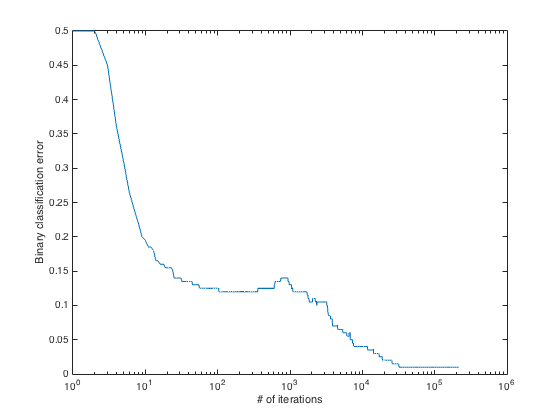
\includegraphics[width=\columnwidth]
    {figures/bin_err.png}
    \caption{\footnotesize{\bf}Binary Classification Error}
    \label{fig:bce}
}
\end{figure}

\begin{figure}[!h]
{
    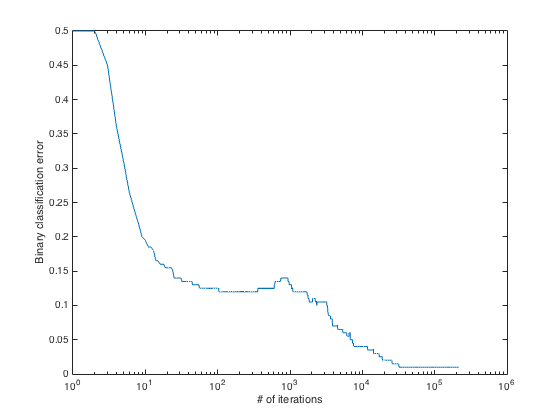
\includegraphics[width=\columnwidth]
    {figures/bin_err.png}
    \caption{\footnotesize{\bf}Empirical Risk}
    \label{fig:er}
}
\end{figure}


For tolerance 0.0001 and step 0.1 the algorithm needs 217797 iterations.



\end{document}

